% =====================================================================
%  Pricing the Unicorn - NFL draft athletic outliers, 2000-2026
%  Compile with pdfLaTeX (Overleaf default). Upload the whole folder:
%     main.tex   figures/*.pdf   tables/*.tex
%  Every number, table and figure is produced by the scripts in code/.
% =====================================================================
\documentclass[11pt]{article}
\usepackage[T1]{fontenc}
\usepackage[utf8]{inputenc}
\usepackage[sc]{mathpazo}
\usepackage[scaled=0.9]{helvet}
\usepackage{courier}
\usepackage[margin=0.95in,top=1in,bottom=1in]{geometry}
\usepackage{microtype}
\usepackage{amsmath,amssymb}
\usepackage{graphicx}
\usepackage{booktabs,tabularx,array,longtable}
\usepackage[table]{xcolor}
\usepackage{caption}
\usepackage{float}
\usepackage{placeins}
\renewcommand{\topfraction}{0.92}\renewcommand{\bottomfraction}{0.85}\renewcommand{\textfraction}{0.06}\renewcommand{\floatpagefraction}{0.8}
\setcounter{topnumber}{3}\setcounter{bottomnumber}{2}\setcounter{totalnumber}{5}
\usepackage{enumitem}
\usepackage{titlesec}
\usepackage{fancyhdr}
\usepackage{listings}
\usepackage[colorlinks=true,linkcolor=ink,citecolor=accent,urlcolor=accent]{hyperref}

% ---------- colours and small macros
\definecolor{ink}{HTML}{22303C}
\definecolor{accent}{HTML}{2A6F97}
\definecolor{stealc}{HTML}{2A9D8F}
\definecolor{bustc}{HTML}{D1495B}
\definecolor{goodc}{HTML}{5F7389}
\definecolor{freakc}{HTML}{C98600}
\definecolor{rule}{HTML}{C9D3DC}
\definecolor{boxbg}{HTML}{F3F6F9}
\newcommand{\steal}{\textcolor{stealc}{\textbf{Steal}}}
\newcommand{\bust}{\textcolor{bustc}{\textbf{Bust}}}
\newcommand{\good}{\textcolor{goodc}{Good value}}
\newcommand{\early}{\textit{Too early}}
\newcommand{\AV}{\mathrm{AV}}
\makeatletter\newcommand{\tabinput}[1]{\@@input #1 }\makeatother  % \input that is safe inside tabular

\linespread{1.02}
\setlength{\parskip}{0.4em}
\setlength{\parindent}{0pt}
\captionsetup{font=small,labelfont={bf,sf},textfont={sf},skip=6pt}
\titleformat{\section}{\Large\sffamily\bfseries\color{ink}}{\thesection}{0.6em}{}
\titleformat{\subsection}{\large\sffamily\bfseries\color{ink}}{\thesubsection}{0.6em}{}
\titlespacing*{\section}{0pt}{1.4em}{0.5em}
\titlespacing*{\subsection}{0pt}{1.0em}{0.3em}
\pagestyle{fancy}\fancyhf{}
\fancyhead[L]{\small\sffamily\color{goodc} Pricing the Unicorn}
\fancyhead[R]{\small\sffamily\color{goodc} NFL Draft, 2000--2026}
\fancyfoot[C]{\small\sffamily\thepage}
\renewcommand{\headrulewidth}{0.3pt}
\setlist{itemsep=0.2em,topsep=0.3em}
\lstset{basicstyle=\ttfamily\scriptsize,keywordstyle=\color{accent}\bfseries,commentstyle=\color{goodc}\itshape,
        stringstyle=\color{freakc},language=Python,frame=single,rulecolor=\color{rule},backgroundcolor=\color{boxbg},
        breaklines=true,columns=fullflexible,showstringspaces=false,xleftmargin=4pt,xrightmargin=4pt}
\newcommand{\takeaway}[1]{\par\smallskip\noindent\colorbox{boxbg}{\parbox{\dimexpr\linewidth-2\fboxsep}{\sffamily\small #1}}\par\smallskip}

\begin{document}
\thispagestyle{empty}

% ---------- title block (add your name on the marked line)
{\sffamily
{\color{accent}\rule{\linewidth}{2pt}}\\[0.9em]
{\Huge\bfseries\color{ink} Pricing the Unicorn}\\[0.5em]
{\Large\color{ink} Unsupervised detection of athletic outliers in the NFL Draft, 2000--2026,\\[0.15em] and what teams got for the picks they spent on them}\\[1.0em]
% {\large Your Name}\\[0.3em]      % <-- uncomment and edit
{\normalsize\color{goodc} Working paper \textbullet\ October 2026}\\[0.4em]
{\color{rule}\rule{\linewidth}{0.6pt}}
}

\begin{abstract}
\noindent Every draft cycle produces a handful of prospects whose bodies and workouts do not look like anyone else's at their position. This paper asks a front-office question about them: \emph{when a team spends a pick on a unicorn, does it get its money's worth?} We take every position player with a timed 40-yard dash from 27 combine classes (2000--2026; $n = 7{,}690$), adjust each drill for size and era, and score how unusual each profile is with an ensemble of three unsupervised detectors (Isolation Forest, Local Outlier Factor and a robust Mahalanobis distance) run position by position. The most anomalous 5\% (390 players) are split by direction into \emph{Freaks} (108), \emph{Odd builds} (134) and \emph{Red flags} (148). We then grade each drafted player from the 2000--2022 classes against a slot-value curve built from Approximate Value, as a \bust, \good\ or \steal.

Three results stand out. First, the league pays heavily for freak athleticism: Freaks are drafted 88\% of the time against 67\% for typical prospects, at a median pick of 66 against 109. Second, at that price they are fairly valued and no more: across 84 graded Freaks the bust rate is 11\% and the steal rate 20\%, against 14\% and 17\% for typical players, a difference well inside sampling noise. Third, the average hides structure. First-round Freaks have out-performed their slot (7\% busts, 37\% steals; $n=27$), while unusually built players taken in rounds 2--3 and outsized offensive tackles have been poor bets. Team-level differences in unicorn drafting are no larger than chance would produce.
\end{abstract}

\vspace{0.3em}
{\sffamily\small\color{goodc}\textbf{Keywords:} anomaly detection, Isolation Forest, NFL Draft, combine, draft value, market efficiency}

\section{Introduction}

Scouts call them unicorns: the 239-pound receiver who runs 4.35, the 341-pound nose tackle who runs 4.78, the 6-foot-4 cornerback who runs 4.26. The term is used loosely, and the players it describes are remembered selectively. Calvin Johnson is remembered. Taylor Mays, who was just as rare a size--speed specimen at safety, mostly is not.

For a team the useful question is not whether unicorns are exciting but whether they are \emph{priced correctly}. A prospect with a one-in-a-hundred body costs a premium pick. If the league systematically over-pays for rarity, the smart move is to let someone else draft the workout warrior. If it under-pays, rarity is a bargain. Answering that requires two things done carefully and separately: a definition of ``unicorn'' that does not peek at NFL outcomes, and a measure of value that accounts for where the player was picked.

This paper builds both.

\begin{enumerate}[leftmargin=1.4em]
\item \textbf{Detection is unsupervised.} We never tell the model who became a good player. Within each position group, three detectors with different notions of ``unusual'' score every prospect's size and workout profile, and we keep the players all three agree are far from the crowd (Section~\ref{sec:methods}).
\item \textbf{Direction is separated from rarity.} Anomaly detectors are direction-blind: a 4.26 corner and a 4.85 corner are equally ``anomalous''. We label each outlier a \emph{Freak}, an \emph{Odd build} or a \emph{Red flag} using a size-adjusted athleticism composite.
\item \textbf{Value is measured against the slot.} A player's career Approximate Value is compared with what his pick, draft class and position would be expected to return, and graded \bust, \good\ or \steal.
\item \textbf{The lens is the team's.} We report what the market pays for unicorns, what it gets back, where the pattern breaks by round, position and body type, and how each of the 32 franchises has fared.
\end{enumerate}

\takeaway{\textbf{Headline.} The NFL draft prices freak athletes about right. They cost roughly 40 picks more than a typical prospect and return roughly what that higher slot implies. The actionable signal is narrower: \emph{elite, confirmed} freaks at the top of round one have been safer than their peers, while \emph{unusual-but-not-athletic} builds on day two have been worse.}

\paragraph{A note on scope.} The request that motivated this project sketched a model mixing athletic measurables with college usage statistics (dominator rating, target share). No open, complete source of college usage covers all positions back to 2000, so this paper restricts itself to what can be measured for every prospect in every class: height, weight and the six combine drills. That makes these \emph{athletic} unicorns. Production unicorns of the Deebo Samuel or Puka Nacua type are outside the model, and Section~\ref{sec:limits} describes how to add them.

\section{Data}\label{sec:data}

\subsection{Sources}

All data come from the open \texttt{nflverse} project \cite{nflverse}, which redistributes Pro-Football-Reference tables:

\begin{itemize}[leftmargin=1.4em]
\item \textbf{Combine file}: 8,968 prospect rows for the 2000--2026 classes, with height, weight, 40-yard dash, bench press, vertical jump, broad jump, three-cone and 20-yard shuttle, plus draft year, round and overall pick where applicable.
\item \textbf{Draft file}: every selection since 1980 with career weighted Approximate Value (AV), games, starts, Pro Bowls and All-Pro selections. We use the 2000--2025 classes for valuation.
\item \textbf{Players file}: NFL roster positions, used only to resolve the generic combine labels (OL, DL, DB) that appear from 2019 onward.
\end{itemize}

Approximate Value \cite{drinen} is Pro-Football-Reference's single-number summary of a player-season, designed to be comparable across positions. The weighted career version counts a player's best season in full and discounts each successive season by five percentage points. It is coarse, but it is the only public measure that covers a guard, a safety and a quarterback on one scale for 26 draft classes.

\subsection{Sample construction}

We drop specialists and fullbacks and assign the remaining prospects to eleven position groups. Outside linebackers are split by weight (245\,lb and above are treated as edge rushers), and generic labels are resolved from NFL roster position where available. A prospect enters the modelling sample if he has a measured height, weight and 40-yard dash; other drills may be missing. Three cleaning steps matter:

\begin{itemize}[leftmargin=1.4em]
\item \textbf{Namesakes.} The source file occasionally assigns one draft pick to two same-named prospects (two Derrick Johnsons in 2005, for instance). We keep the row whose position matches the drafted player and drop the other.
\item \textbf{Mislabelled rows.} An anomaly detector's first discoveries are always data errors. Nine rows had a size that is impossible for the listed position (a 195-lb ``offensive lineman'', a 305-lb ``linebacker''), most of them from the 2021 pro-day class. They are removed by narrow rules (linemen under 270\,lb, linebackers outside 210--275\,lb) so that genuine size outliers such as 370-lb tackles remain.
\item \textbf{The 2021 class.} There was no 2021 combine. That year's numbers are pro-day results, which are hand-timed and flattering, so each drill receives a 2021-specific shift in the adjustment regression described below.
\end{itemize}

Table~\ref{tab:sample} summarises the final sample of 7,690 prospects, of whom 5,081 were drafted and 4,526 belong to the 2000--2022 classes that are old enough to grade. The average prospect completed 4.6 of the six drills; 24\% of drill cells are missing and are imputed.

\begin{table}[!htb]
\centering\small\sffamily
\caption{Modelling sample by position group. ``Graded'' = drafted in 2000--2022. Unicorns are the top 5\% of the consensus anomaly score within each position. The right-hand block gives the share of prospects with a recorded result in each non-40 drill.}
\label{tab:sample}
\begin{tabular}{l rrr r rrr rrrrr}
\toprule
 & \multicolumn{3}{c}{Prospects} & \multicolumn{4}{c}{Unicorns} & \multicolumn{5}{c}{Drill coverage (\%)}\\
\cmidrule(lr){2-4}\cmidrule(lr){5-8}\cmidrule(lr){9-13}
Group & All & Drafted & Graded & All & Freak & Odd & Red & Bench & Vert & Broad & Cone & Shut \\
\midrule
\tabinput{tables/sample.tex}
\bottomrule
\end{tabular}
\end{table}

\section{Methods}\label{sec:methods}

\subsection{Size- and era-adjusted features}

Raw drill results are dominated by body size: a 4.9-second 40 is slow for a receiver and remarkable for a nose tackle. Splitting by position removes most of this, but within a position weight still explains much of the variance. For each position group $g$ and drill $d$ we therefore fit, on the prospects who actually performed the drill,
\begin{equation}
x_{id} \;=\; \beta_0 + \beta_1\,\mathrm{ht}_i + \beta_2\,\mathrm{wt}_i + \beta_3\,\mathrm{wt}_i^2 + \beta_4\,(\mathrm{year}_i-2013) + \beta_5\,\mathbf{1}[\mathrm{year}_i=2021] + \varepsilon_{id},
\end{equation}
and take the residual, scaled robustly and oriented so that positive is always better:
\begin{equation}
a_{id} \;=\; s_d\,\frac{\hat\varepsilon_{id}-\mathrm{median}(\hat\varepsilon_{d})}{1.4826\,\mathrm{MAD}(\hat\varepsilon_{d})},\qquad s_d=\begin{cases}-1 & \text{timed drills (40, cone, shuttle)}\\ +1 & \text{bench, vertical, broad jump.}\end{cases}
\end{equation}
The value $a_{i,40}=+2$ means ``two robust standard deviations faster than a player of this height, weight and class year is expected to run''. Height and weight themselves enter as robust $z$-scores within position. The feature vector is thus
$\mathbf{f}_i=(z^{\mathrm{ht}}_i,\,z^{\mathrm{wt}}_i,\,a_{i,40},\,a_{i,\mathrm{bench}},\,a_{i,\mathrm{vert}},\,a_{i,\mathrm{broad}},\,a_{i,\mathrm{cone}},\,a_{i,\mathrm{shuttle}})$, with bench omitted for quarterbacks because only 5\% of them lift.

Medians and MADs are used instead of means and standard deviations so that the very outliers we are looking for do not inflate the yardstick used to find them.

\subsection{Missing drills}

Prospects skip drills strategically, so deleting incomplete rows would discard the most interesting players: the source file records only a height, a weight and a 40 time for Calvin Johnson. Missing drills are filled by chained-equations imputation \cite{mice} within position (scikit-learn's \texttt{IterativeImputer} with Bayesian ridge regressions \cite{sklearn}). Each imputed value is a conditional mean, so it sits near the centre of the distribution given the player's other measurements. Imputation therefore makes a player look \emph{less} unusual, never more; it is conservative with respect to flagging.

That conservatism has a cost, which motivates the second view below: a player with one spectacular measured result and five imputed ones is dragged toward the middle.

\subsection{Three detectors}

No single algorithm owns the definition of ``outlier'', so we use three with different geometries.

\textbf{Isolation Forest} \cite{iforest} builds random trees that split on a random feature at a random threshold. Unusual points are isolated in few splits. With $h(\mathbf{f})$ the path length to isolate a point, averaged over 500 trees, and $c(n)$ the expected path length in a sample of size $n$, the score is
\begin{equation}
s_{\mathrm{IF}}(\mathbf{f}) = 2^{-\,\mathbb{E}[h(\mathbf{f})]/c(n)} .
\end{equation}
It is good at catching extreme values on individual axes and is the method in the sketch that inspired this project.

\textbf{Local Outlier Factor} \cite{lof} compares the density around a point with the density around its $k$ nearest neighbours ($k=35$):
\begin{equation}
s_{\mathrm{LOF}}(\mathbf{f}) = \frac{1}{k}\sum_{\mathbf{o}\in N_k(\mathbf{f})}\frac{\mathrm{lrd}_k(\mathbf{o})}{\mathrm{lrd}_k(\mathbf{f})},
\end{equation}
where $\mathrm{lrd}_k$ is local reachability density. It catches players who sit in an empty pocket of the space even when no single measurement is extreme.

\textbf{Robust Mahalanobis distance} measures distance from the centre in units that respect the correlations between drills,
\begin{equation}
s_{\mathrm{MD}}(\mathbf{f}) = \sqrt{(\mathbf{f}-\hat{\boldsymbol\mu})^{\!\top}\hat{\boldsymbol\Sigma}^{-1}(\mathbf{f}-\hat{\boldsymbol\mu})},
\end{equation}
with $\hat{\boldsymbol\mu},\hat{\boldsymbol\Sigma}$ from the Minimum Covariance Determinant estimator \cite{mcd}, which fits location and scatter to the most concentrated 85\% of the data. It penalises \emph{unusual combinations}: fast but not explosive, heavy but short.

\subsection{Two views and a consensus score}

Each detector is run on two feature sets per position: the \textbf{full-workout view} (all eight features, imputed where needed) and the \textbf{size--speed view} (height, weight and adjusted 40 only, which every player has measured). Within each view, the three detector scores are converted to within-position percentile ranks and averaged; a player's consensus score is the higher of his two view scores, re-ranked within position:
\begin{equation}
C_i=\operatorname{rank}_g\!\Big(\max\big\{\,\overline{p}^{\,\mathrm{full}}_i,\ \overline{p}^{\,\mathrm{core}}_i\big\}\Big),\qquad \overline{p}^{\,v}_i=\tfrac13\big(p^{\,v}_{i,\mathrm{IF}}+p^{\,v}_{i,\mathrm{LOF}}+p^{\,v}_{i,\mathrm{MD}}\big).
\end{equation}
A prospect is a \textbf{unicorn} if $C_i>0.95$. The sketch used a contamination rate of 2\%; we use 5\% for statistical power and report 2\% and 10\% as sensitivity checks. Because ranking is within position, every group contributes the same share of unicorns by construction.

\subsection{Direction: Freak, Odd build, Red flag}

The athleticism composite is the mean of a player's oriented drill scores, standardised within position, $A_i = \operatorname{std}_g\!\big(\tfrac1{|D|}\sum_{d\in D} a_{id}\big)$. Unicorns are then typed:
\begin{center}\small\sffamily
\begin{tabular}{lll}
\toprule
Type & Rule & Reading\\
\midrule
\textcolor{freakc}{\textbf{Freak}} & $C_i>0.95$ and $A_i\ge +0.75$ & Rare \emph{and} clearly more athletic than his size predicts\\
\textbf{Odd build} & $C_i>0.95$ and $|A_i|<0.75$ & Rare mainly through body dimensions or a mixed profile\\
\textcolor{bustc}{\textbf{Red flag}} & $C_i>0.95$ and $A_i\le -0.75$ & Rare because he tested far below his size peers\\
\bottomrule
\end{tabular}
\end{center}

\subsection{The slot-value model and the three grades}\label{sec:value}

Expected career value is modelled multiplicatively,
\begin{equation}
\mathbb{E}[\AV_i] \;=\; f(\mathrm{pick}_i)\times g(\mathrm{class}_i)\times m(\mathrm{pos}_i).
\end{equation}

\begin{itemize}[leftmargin=1.4em]
\item $f(\cdot)$ is a LOWESS smooth \cite{lowess} of career AV on log pick for the mature 2000--2015 classes, constrained to be non-increasing. It falls from 68 AV at pick 1 to 47 at pick 10, 35 at pick 32, 16 at pick 100 and 6 at pick 250, in line with the steep-then-flat shape found by Massey and Thaler \cite{massey}.
\item $g(\cdot)$ is a class factor: the class's realised AV divided by what $f$ implies. It is close to one for finished classes and falls to 0.88, 0.80, 0.67 and 0.61 for the 2019--2022 classes, whose careers are still in progress. This puts a four-year veteran and a retired player on the same footing.
\item $m(\cdot)$ is a position multiplier, because AV is more generous to some positions: 1.36 for interior linemen and 1.16 for tackles down to 0.87 for receivers, 0.81 for cornerbacks and 0.68 for tight ends.
\end{itemize}

The spread around expectation, $\sigma(\mathrm{pick})$, is a LOWESS smooth of squared residuals scaled by the same $g$ and $m$. Each player then has a value over expected, $\mathrm{VOE}_i=\AV_i-\mathbb{E}[\AV_i]$, a standardised version $z_i=\mathrm{VOE}_i/\sigma_i$, and a ratio $r_i=\AV_i/\mathbb{E}[\AV_i]$. The grades are:
\begin{center}\small\sffamily
\begin{tabular}{ll}
\toprule
\steal & $z_i\ge +0.75$ and $r_i\ge 1.5$ \quad (well above the slot and at least 50\% more than expected)\\
\bust & $z_i\le -0.75$ and $r_i< 0.5$ \quad (well below the slot and less than half of what was expected)\\
\good & everything in between\\
\bottomrule
\end{tabular}
\end{center}
Classes after 2022 have fewer than four completed seasons and are marked \early.

Requiring both a standardised and a proportional condition has a deliberate consequence. A seventh-round pick who never plays is not a bust, because almost nothing was expected of him: his $z$ cannot reach $-0.75$. Across all 5,769 position players drafted in 2000--2022 the scheme labels 12\% busts, 71\% good value and 17\% steals; busts run at 20--24\% in rounds 1--4 and essentially zero after, while steals run at 13--18\% in every round (Figure~\ref{fig:curve}).

\begin{figure}[!htb]
\centering
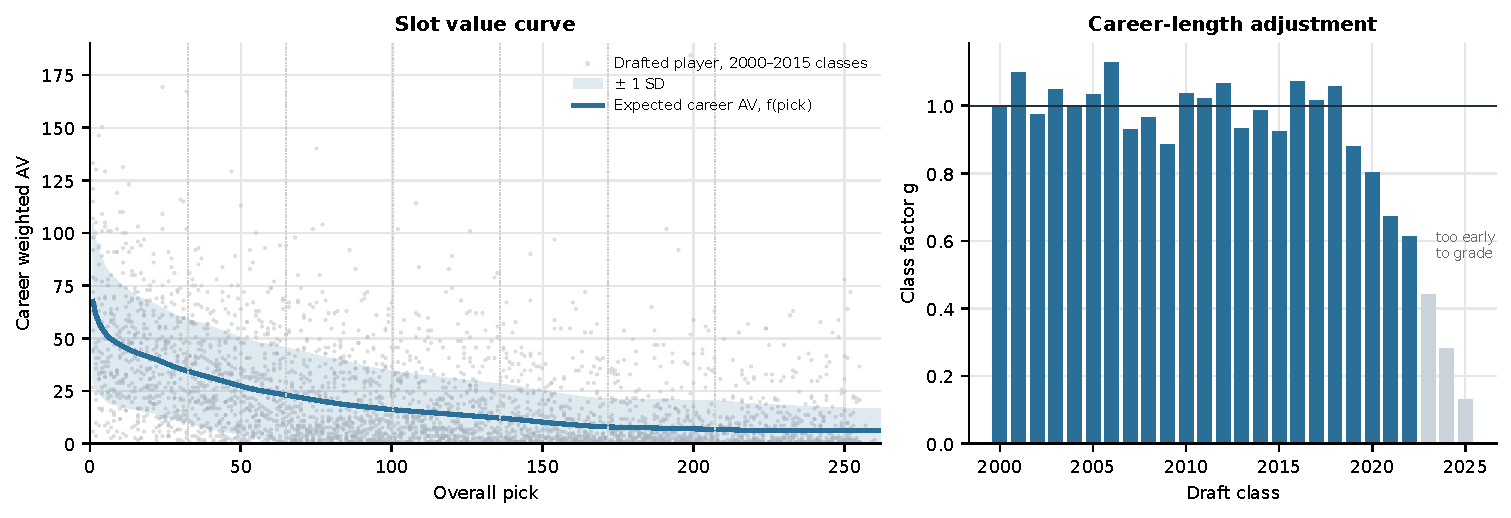
\includegraphics[width=\linewidth]{figures/fig_valuecurve.pdf}
\caption{Left: career weighted AV by overall pick for the 2000--2015 classes with the fitted slot curve $f$ and a one-SD band. Right: the class factor $g$ that rescales expectations for classes whose careers are unfinished.}
\label{fig:curve}
\end{figure}

\subsection{Inference}

Because $z$ already nets out pick, class and position, the main comparison is simply mean $z$ by unicorn type, with percentile bootstrap intervals (4,000 resamples). We add Welch $t$-tests and Mann--Whitney tests against typical players, $\chi^2$ and Fisher exact tests on grade shares, and an OLS regression of $z$ on type with log-pick, position and class fixed effects and heteroskedasticity-robust errors. Team-level skill is tested by permuting franchise labels.

\section{Who the unicorns are}\label{sec:who}

\subsection{What the detectors find}

Figure~\ref{fig:sizespeed} shows the most intuitive slice of the feature space. In each panel the grey cloud is the position's normal range and the coloured points are flagged players. The receivers in the upper right are the classic case: Calvin Johnson at 239\,lb and 4.35, D.K.\ Metcalf at 228 and 4.33, Vincent Jackson at 241 and 4.46. But the flags are not confined to that corner. Small, extremely fast players are flagged too, as are heavy, slow ones, and the colour (not the position on the plot alone) says which kind of rare each is.

\begin{figure}[!htb]
\centering
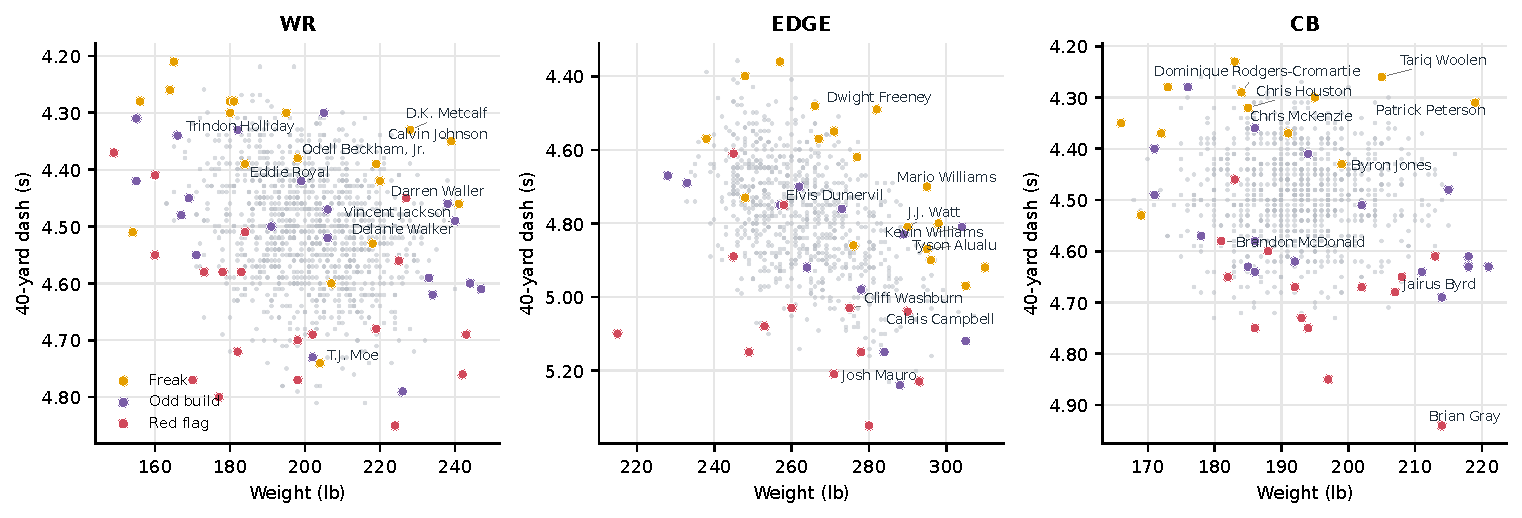
\includegraphics[width=\linewidth]{figures/fig_sizespeed.pdf}
\caption{Weight against 40 time for three position groups (faster is up). Grey: typical prospects. Coloured: unicorns by type. Some flagged players sit inside the cloud here because they are unusual on other drills.}
\label{fig:sizespeed}
\end{figure}

Figure~\ref{fig:pca} projects the full feature set for six positions onto its first two principal components. Unicorns form a ring around the central mass. Freaks and Red flags tend to sit at opposite ends of the first component, which in every position is a general athleticism axis; Odd builds sit off-axis, where body dimensions dominate.

\begin{figure}[!htb]
\centering
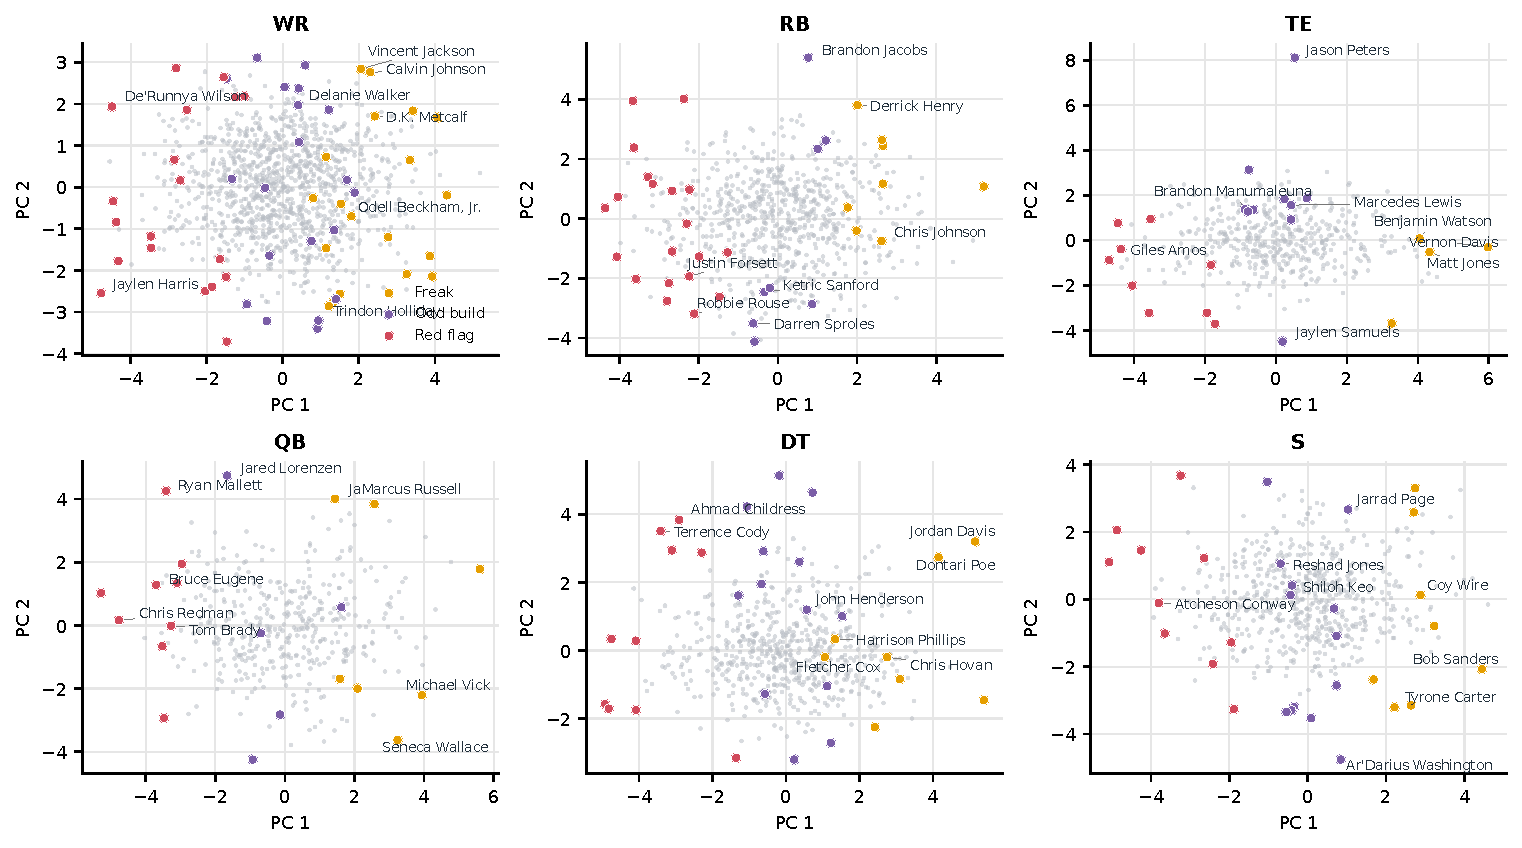
\includegraphics[width=0.88\linewidth]{figures/fig_pca.pdf}
\caption{First two principal components of the adjusted features for six position groups. The detectors work in the full eight-dimensional space; this is a two-dimensional shadow of it.}
\label{fig:pca}
\end{figure}

\subsection{Do the detectors agree?}

Largely, but not entirely, which is the reason to use three. In the full-workout view the rank correlations between detector scores are 0.88 (Isolation Forest and LOF), 0.91 (Isolation Forest and Mahalanobis) and 0.94 (LOF and Mahalanobis). At the tails the agreement is looser (Figure~\ref{fig:detectors}): of the 541 players that at least one detector puts in its top tier, 155 are put there by all three. The two views differ more than the detectors do. Each view flags about 390 players at the 5\% level, and only 142 are flagged by both, which confirms that the size--speed view recovers players the imputed full view misses.

\begin{figure}[!htb]
\centering
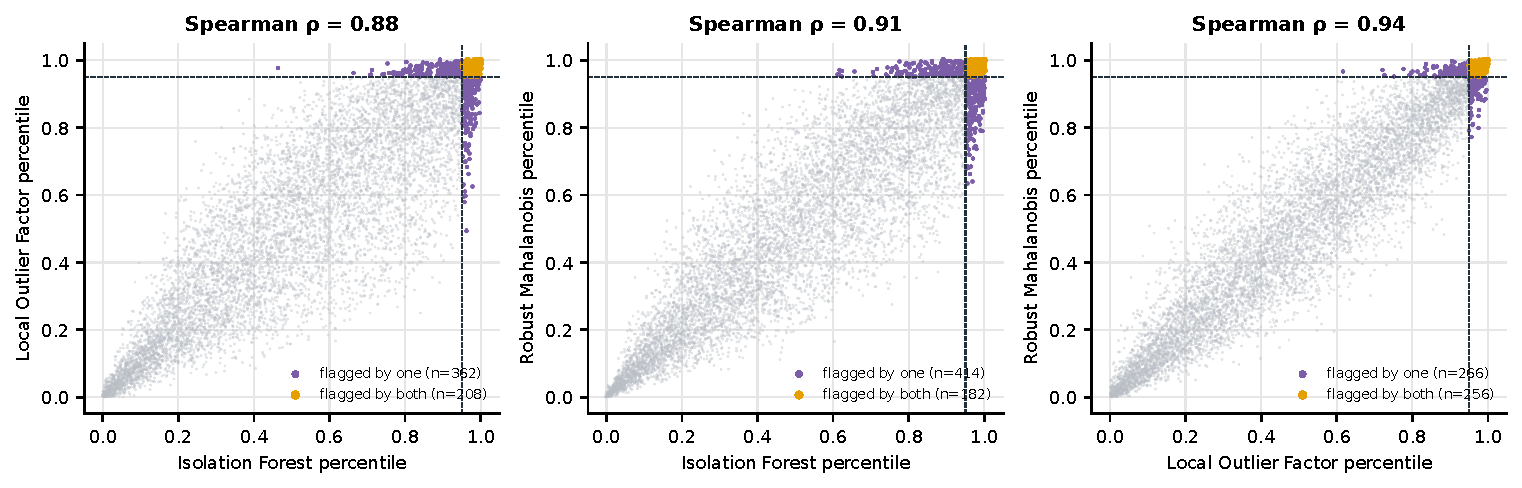
\includegraphics[width=0.9\linewidth]{figures/fig_detectors.pdf}
\caption{Pairwise agreement between detectors (full-workout view, within-position percentiles). Dashed lines mark the 95th percentile.}
\label{fig:detectors}
\end{figure}

\subsection{The census}

The model flags 390 unicorns across 27 classes: 108 Freaks, 134 Odd builds and 148 Red flags. Outside 2021 the count runs between 5 and 26 a year and is lower in recent classes (Figure~\ref{fig:perclass}). The 2021 spike of 43 is a sample-composition effect rather than a talent effect: without a combine, that year's file contains more than 360 pro-day participants, many of whom would never have been invited to Indianapolis. Most of them are undrafted Red flags and do not enter the value analysis.

\begin{figure}[!htb]
\centering
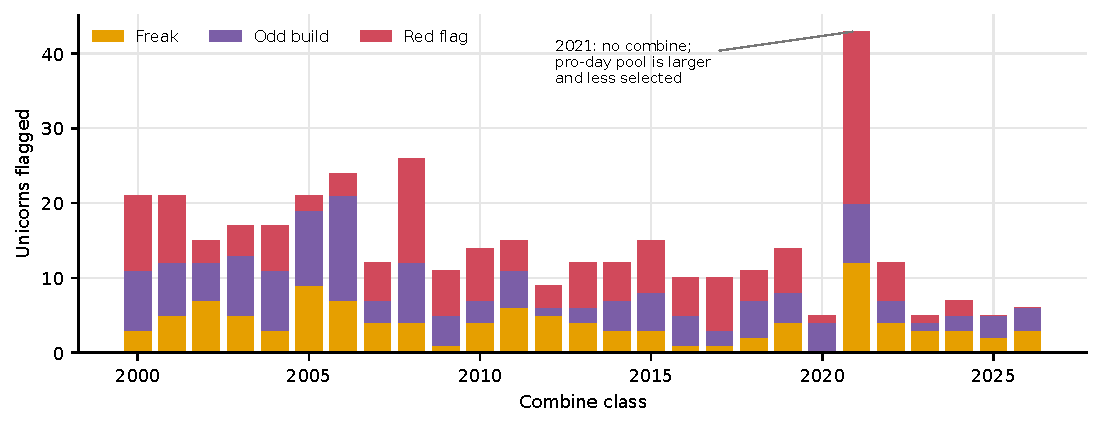
\includegraphics[width=0.66\linewidth]{figures/fig_perclass.pdf}
\caption{Unicorns flagged per combine class, by type.}
\label{fig:perclass}
\end{figure}

Table~\ref{tab:top} lists the 25 highest-scoring drafted Freaks from gradeable classes. The list reads like a scout's memory of rare bodies: Jordan Davis, Tariq Woolen, Mario Williams, Metcalf, Dontari Poe, Patrick Peterson, Calvin Johnson. It also contains JaMarcus Russell (a 265-lb quarterback who ran 4.83), Mike Williams (a 375-lb tackle) and a long tail of day-three picks who never started. An unsupervised model has no way to know which is which, and that is the point of grading them afterwards.

\begin{table}[!htb]
\centering\footnotesize\sffamily
\setlength{\tabcolsep}{3.6pt}
\caption{The 25 most anomalous drafted Freaks, 2000--2022 classes, ordered by consensus score. Ath = athleticism composite (SD within position). E[AV] = slot expectation. Team codes follow Pro-Football-Reference (GNB, KAN, NWE, SFO, TAM, NOR, LVR, LAC, LAR; relocated franchises are folded into their current identity). Positions are as listed at the combine.}
\label{tab:top}
\begin{tabular}{llr rrr r rl rrr l}
\toprule
Player & Pos & Class & Ht & Wt & 40 & Ath & Pick & Team & AV & E[AV] & $z$ & Grade\\
\midrule
\tabinput{tables/top_freaks.tex}
\bottomrule
\end{tabular}
\end{table}

\subsection{Five archetypes}

To describe \emph{how} unicorns are unusual we cluster the 390 flagged players with $k$-means on six summary dimensions (height, weight, adjusted speed, explosion, agility, strength). Silhouette scores decline gently from 0.25 at $k=3$ to 0.21 at $k=5$ and are low throughout, so these are regions of a continuum rather than crisp species; we use $k=5$ because the five centres are easy to read (Figure~\ref{fig:arch}, Table~\ref{tab:arch}).

\begin{figure}[!htb]
\centering
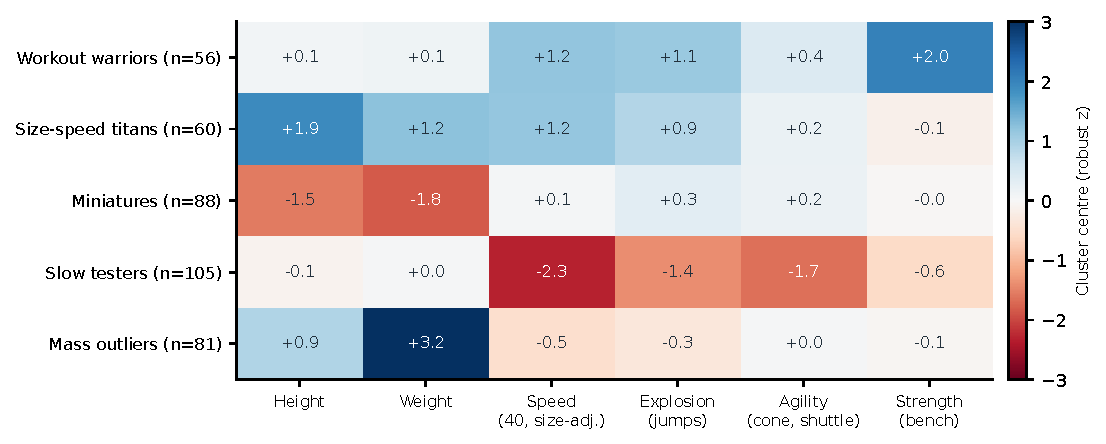
\includegraphics[width=0.7\linewidth]{figures/fig_archetypes.pdf}
\caption{Cluster centres of the five unicorn archetypes, in robust SD units within position. Blue is above the positional norm, red below.}
\label{fig:arch}
\end{figure}

\begin{table}[!htb]
\centering\footnotesize\sffamily
\setlength{\tabcolsep}{3.5pt}
\caption{Archetype outcomes. $n$ = all flagged; Graded = drafted 2000--2022. Examples are the five highest-AV members.}
\label{tab:arch}
\begin{tabularx}{\linewidth}{l rr r r rr l X}
\toprule
Archetype & $n$ & Graded & Ath & Mean $z$ & Steal & Bust & Most common & Examples\\
\midrule
\tabinput{tables/archetypes.tex}
\bottomrule
\end{tabularx}
\end{table}

The two archetypes that correspond to what scouts mean by ``unicorn'' are the \emph{Size--speed titans} (tall, heavy and fast: Peterson, Henry, Calvin Johnson, Parsons) and the \emph{Workout warriors} (normal frame, elite across speed, jumps and bench: Watt, Cox, Freeney, Metcalf, Vernon Davis). Both have returned modestly more than their slots, with bust rates of 7--10\%. The \emph{Mass outliers}, players whose defining trait is being far heavier than their position, are the one archetype with a clearly elevated bust rate (24\%). The \emph{Slow testers} have a high mean only because one of their 25 graded members is Tom Brady.

\section{What the market pays for a unicorn}\label{sec:premium}

Before asking what unicorns return, it is worth measuring what they cost (Figure~\ref{fig:premium}).

\begin{figure}[!htb]
\centering
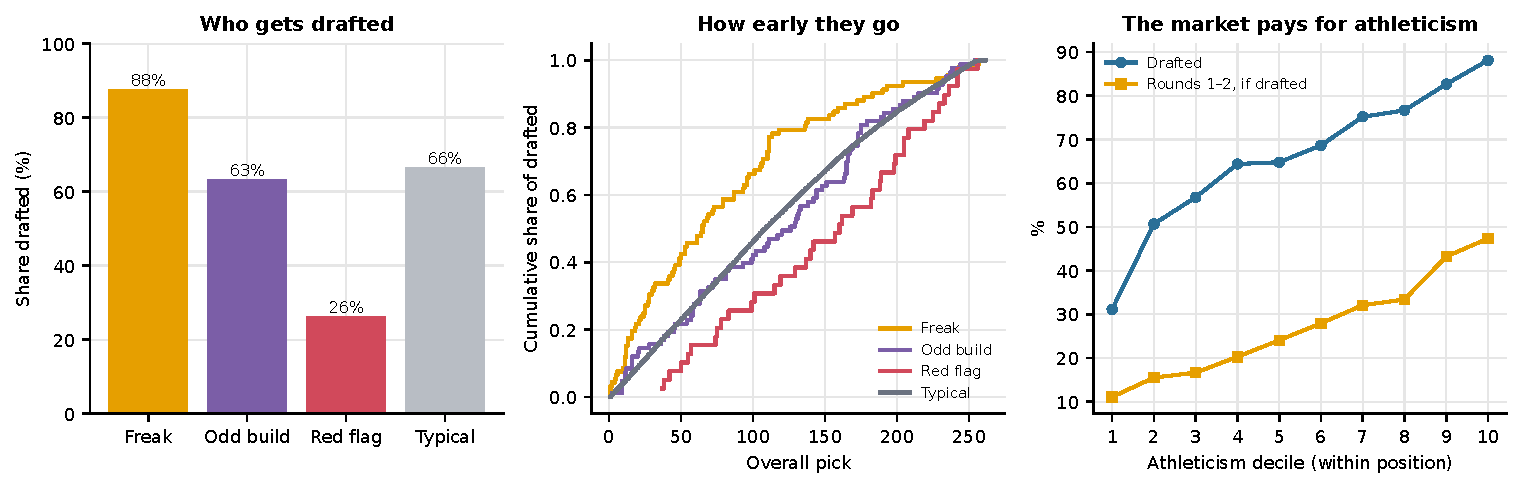
\includegraphics[width=\linewidth]{figures/fig_premium.pdf}
\caption{Left: share of combine prospects drafted, by type (2000--2025 classes). Centre: cumulative distribution of overall pick among those drafted. Right: draft outcomes by decile of the athleticism composite for all prospects.}
\label{fig:premium}
\end{figure}

\begin{itemize}[leftmargin=1.4em]
\item \textbf{Freaks are almost always drafted, and early.} 88\% are selected, against 67\% of typical prospects. Among those drafted the median Freak goes at pick 66 and the median typical prospect at 109; a third of drafted Freaks (33\%) go in round one, against 15\%.
\item \textbf{Red flags are mostly passed over.} Only 26\% are drafted, none in the first round, at a median pick of 160.
\item \textbf{Odd builds are priced like everyone else}: 63\% drafted, median pick 119.
\end{itemize}

The relationship is not confined to the extremes. Across all prospects, a one-SD increase in the athleticism composite multiplies the odds of being drafted by 2.2 (logit coefficient 0.78, $p<0.001$, position fixed effects) and, among the drafted, moves a player up the board by about 26\% of his pick number (coefficient on log pick $-0.31$, $p<0.001$).

Holding athleticism fixed, \emph{rarity itself is not priced}. The anomaly percentile has no relationship with pick ($p=0.81$) and a negative one with being drafted at all (logit coefficient $-0.48$, $p<0.001$). Teams pay for better, not for different.

\takeaway{\textbf{For the draft room.} A Freak costs about 40 picks more than a typical prospect at the median. Any claim that unicorns are ``steals'' has to clear that higher bar. The grades below already do: they compare each player with the expectation for the slot where he was actually taken.}

\section{What teams got: bust, good value, or steal}\label{sec:results}

\subsection{Overall}

Table~\ref{tab:value} and Figure~\ref{fig:grades} give the central result. Of the 201 drafted unicorns from gradeable classes, 31 are steals (15\%), 146 good value (73\%) and 24 busts (12\%).

\begin{table}[!htb]
\centering\small\sffamily
\caption{Value relative to draft slot by unicorn type, drafted players from the 2000--2022 classes. $z$ = value over slot expectation in SD units; CI = 95\% percentile bootstrap.}
\label{tab:value}
\begin{tabular}{l r r rr r r rr rrr}
\toprule
 & & Median & \multicolumn{2}{c}{Mean career AV} & Mean & Mean & \multicolumn{2}{c}{95\% CI for $z$} & \multicolumn{3}{c}{Grade share}\\
\cmidrule(lr){4-5}\cmidrule(lr){8-9}\cmidrule(lr){10-12}
Type & $n$ & pick & Actual & Expected & VOE & $z$ & Low & High & Bust & Good & Steal\\
\midrule
\tabinput{tables/value_by_type.tex}
\bottomrule
\end{tabular}
\end{table}

\begin{figure}[!htb]
\centering
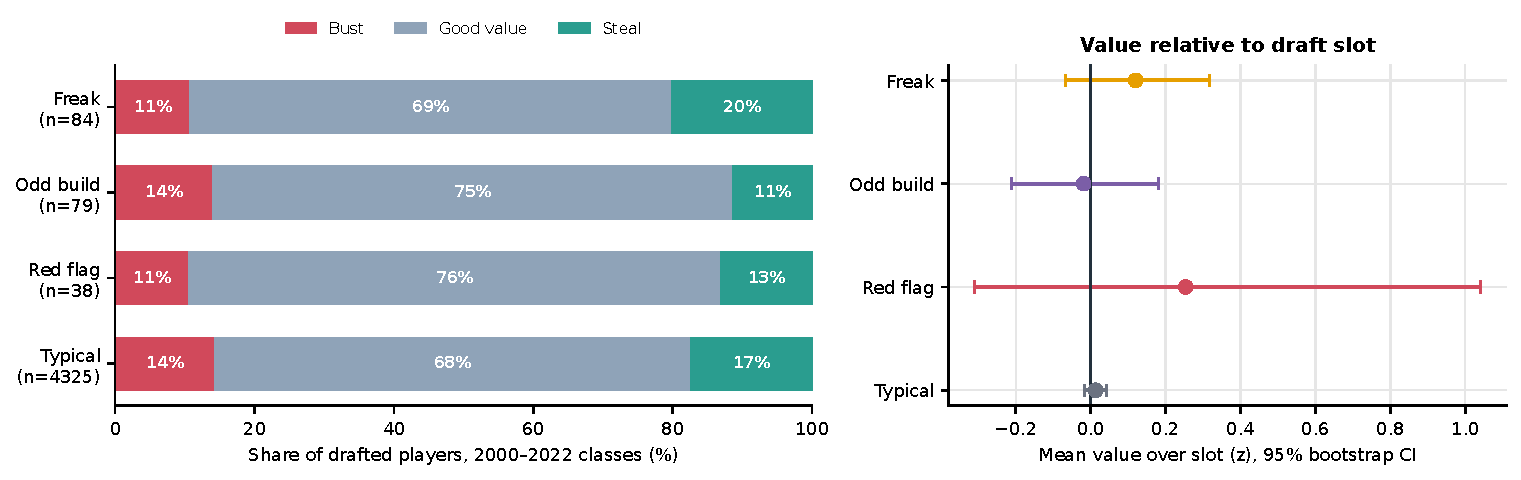
\includegraphics[width=\linewidth]{figures/fig_grades.pdf}
\caption{Left: grade shares by type. Right: mean standardised value over slot with 95\% bootstrap intervals.}
\label{fig:grades}
\end{figure}

\textbf{Freaks} average 28.2 career AV against an expectation of 25.6: $+2.6$ AV, or $+0.12$ SD, with an interval of $-0.08$ to $+0.32$ that comfortably includes zero. Their bust rate is 11\% and their steal rate 20\%, against 14\% and 17\% for typical players. Neither the mean difference (Welch $p=0.29$; Mann--Whitney $p=0.12$) nor the difference in grade mix ($\chi^2$ $p=0.58$) is statistically distinguishable from nothing. A regression with log-pick, position and class fixed effects gives the same answer (Table~\ref{tab:reg}).

\textbf{Odd builds} are indistinguishable from typical players on average ($z=-0.02$).

\textbf{Red flags} show a positive mean ($+0.25$) with a very wide interval. It is one player. Tom Brady ran 5.28 with a 24.5-inch vertical, is correctly flagged as a negative athletic outlier among quarterbacks, and has a $z$ of $+12.8$. Without him the mean for drafted Red flags is $-0.09$. Calais Campbell ($+3.8$) is the other famous member. The honest reading is that the drafted Red flags are a heavily selected group: three in four were not drafted at all, and those who were had something on tape that outweighed the workout.

Median $z$ is negative for every group ($-0.10$ for Freaks, $-0.31$ for typical players) because career value is right-skewed: most picks fall a little short of a mean that is pulled up by a few stars.

\begin{table}[!htb]
\centering\small\sffamily
\caption{OLS regressions of value over slot ($z$) for 4,526 graded players. Both models include log pick and position and draft-class fixed effects; HC1 standard errors.}
\label{tab:reg}
\begin{tabular}{l rrr rrr}
\toprule
 & \multicolumn{3}{c}{Model 1: unicorn type} & \multicolumn{3}{c}{Model 2: continuous scores}\\
\cmidrule(lr){2-4}\cmidrule(lr){5-7}
 & Coef. & SE & $p$ & Coef. & SE & $p$\\
\midrule
\tabinput{tables/regression.tex}
\bottomrule
\end{tabular}
\end{table}

Model 2 is the cleanest summary of the whole paper. Athleticism carries a small positive return \emph{beyond} what the pick already reflects: $+0.037$ SD of slot value per SD of athleticism ($p=0.04$), so the market slightly under-pays for it. Rarity as such carries none ($p=0.18$), and the two do not interact ($p=0.87$). Figure~\ref{fig:deciles} shows both relationships across the whole population.

\begin{figure}[!htb]
\centering
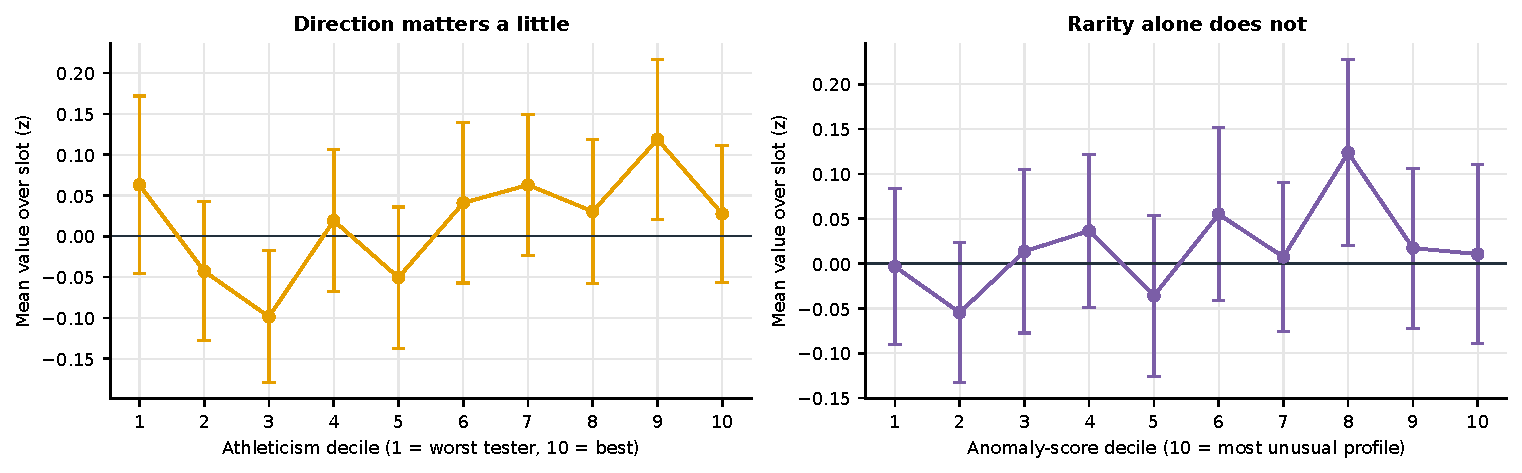
\includegraphics[width=\linewidth]{figures/fig_deciles.pdf}
\caption{Mean value over slot by decile of the athleticism composite (left) and of the consensus anomaly score (right), all graded players. Bars are $\pm1.96$ standard errors.}
\label{fig:deciles}
\end{figure}

\subsection{It depends on the round}

The flat average conceals a pattern by draft capital (Table~\ref{tab:rounds}, Figure~\ref{fig:rounds}).

\begin{table}[!htb]
\centering\small\sffamily
\caption{Value over slot by round and type. Cells with fewer than eight players are omitted.}
\label{tab:rounds}
\begin{tabular}{ll r rr rr}
\toprule
Round & Type & $n$ & Mean VOE (AV) & Mean $z$ & Bust & Steal\\
\midrule
\tabinput{tables/rounds.tex}
\bottomrule
\end{tabular}
\end{table}

\begin{figure}[!htb]
\centering
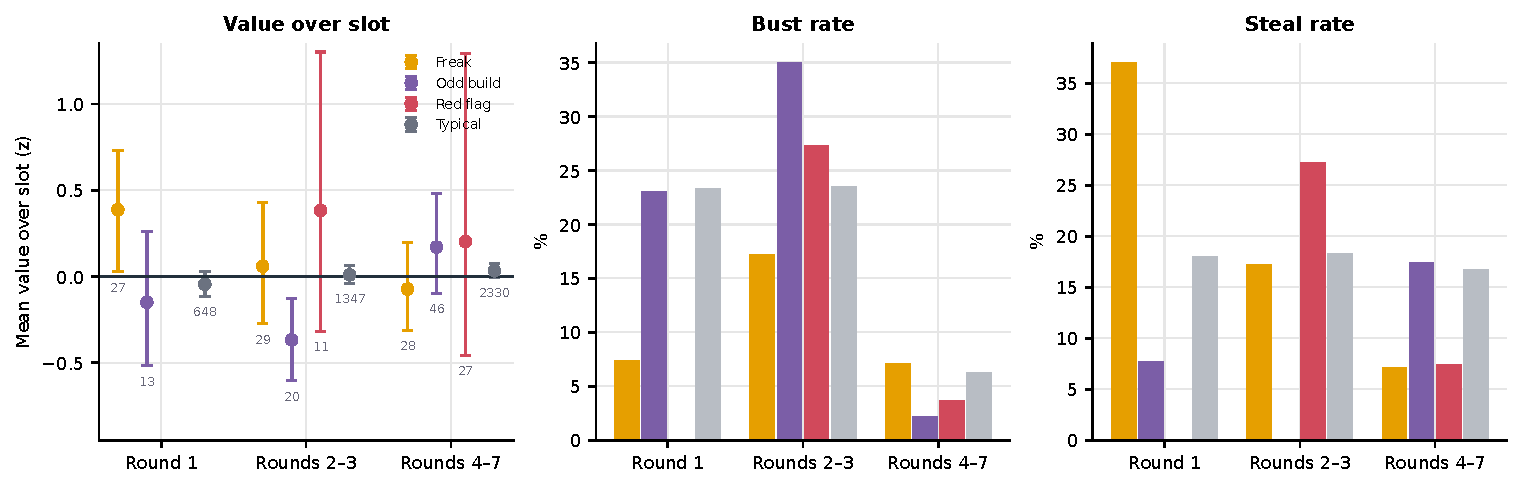
\includegraphics[width=\linewidth]{figures/fig_rounds.pdf}
\caption{Value over slot, bust rate and steal rate by round bucket and type. Small numbers under the intervals are sample sizes; the Red-flag interval in rounds 2--3 ($n=11$) extends beyond the plotted range.}
\label{fig:rounds}
\end{figure}

\textbf{First-round Freaks have beaten their slot.} The 27 Freaks taken in round one average $+9.4$ AV over expectation ($z=+0.39$, bootstrap interval $+0.03$ to $+0.74$; Welch $p=0.03$ against other first-rounders). Two were busts, JaMarcus Russell and the tackle Mike Williams, a rate of 7\% against 23\% for typical first-rounders (Fisher $p=0.06$). Ten were steals (37\% against 18\%, $p=0.02$): Peterson, Watt, Parsons, Chris Johnson, Cox, Freeney, Calvin Johnson, Benjamin Watson, Rodgers-Cromartie and Beckham. A plausible reading is that a Freak only reaches round one when the tape also checks out, and athletic rarity then acts as a floor: a player that much more athletic than his peers finds a role even if he never becomes what was projected.

\textbf{Day-two Odd builds have been the worst cell.} Of 20 Odd builds taken in rounds 2--3, seven were busts and none was a steal ($z=-0.37$). This is the profile of a player drafted on a rare frame without the athletic testing to go with it.

\textbf{Late-round Freaks have not been lottery tickets.} The 28 taken in rounds 4--7 returned slightly less than their slots ($z=-0.07$), with a steal rate of 7\% against 17\% for typical late picks. Tariq Woolen is the exception, not the rule. When a rare athlete is still on the board on day three, the league usually has a reason.

These are subgroup findings from one sample, examined after the overall result came back flat. They should be treated as hypotheses with supporting evidence, not as established effects.

\subsection{It depends on the position}

Figure~\ref{fig:positions} breaks the 201 graded unicorns out by position. Samples are small and only the broad shape should be trusted.

\begin{figure}[!htb]
\centering
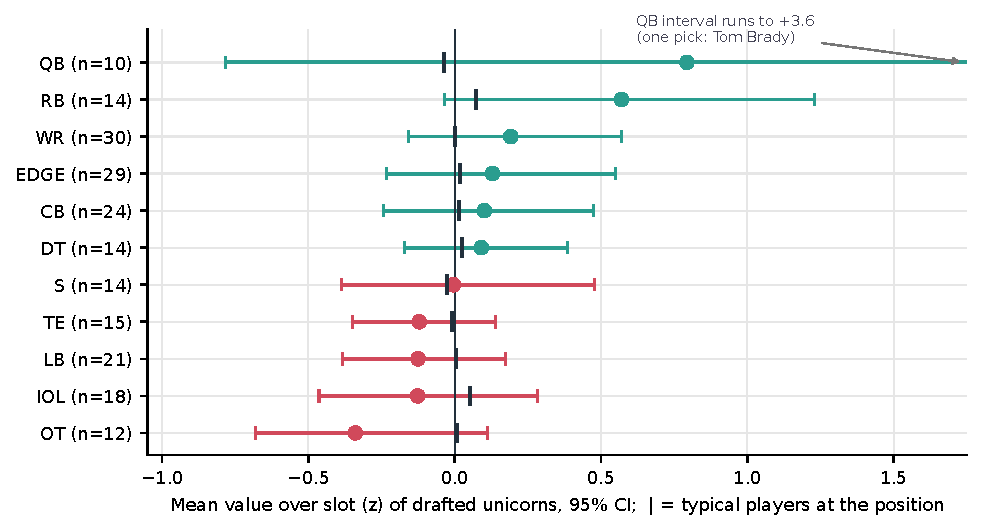
\includegraphics[width=0.68\linewidth]{figures/fig_positions.pdf}
\caption{Mean value over slot of drafted unicorns by position group, with 95\% bootstrap intervals. The vertical tick is the mean for typical players at the same position.}
\label{fig:positions}
\end{figure}


Unicorn running backs (Henry, Chris Johnson, Sproles, Brandon Jacobs) and receivers have done best among positions with a meaningful sample; five of fourteen unicorn backs were steals. The quarterback figure is Brady again. At the other end, \textbf{five of the twelve unicorn offensive tackles were busts}. Ten of the twelve are flagged for mass, at 343\,lb or more, and that group includes Mike Williams, Mekhi Becton and Stockar McDougle against a single clear hit in Orlando Brown. This matches the Mass-outlier archetype result and is the most consistent negative signal in the data: extreme weight at a position is a different thing from extreme athleticism, and it has not aged well.

\subsection{The players}

Figure~\ref{fig:map} places every graded unicorn by pick and career value, and Tables~\ref{tab:steals} and \ref{tab:busts} list the extremes.

\begin{figure}[!htb]
\centering
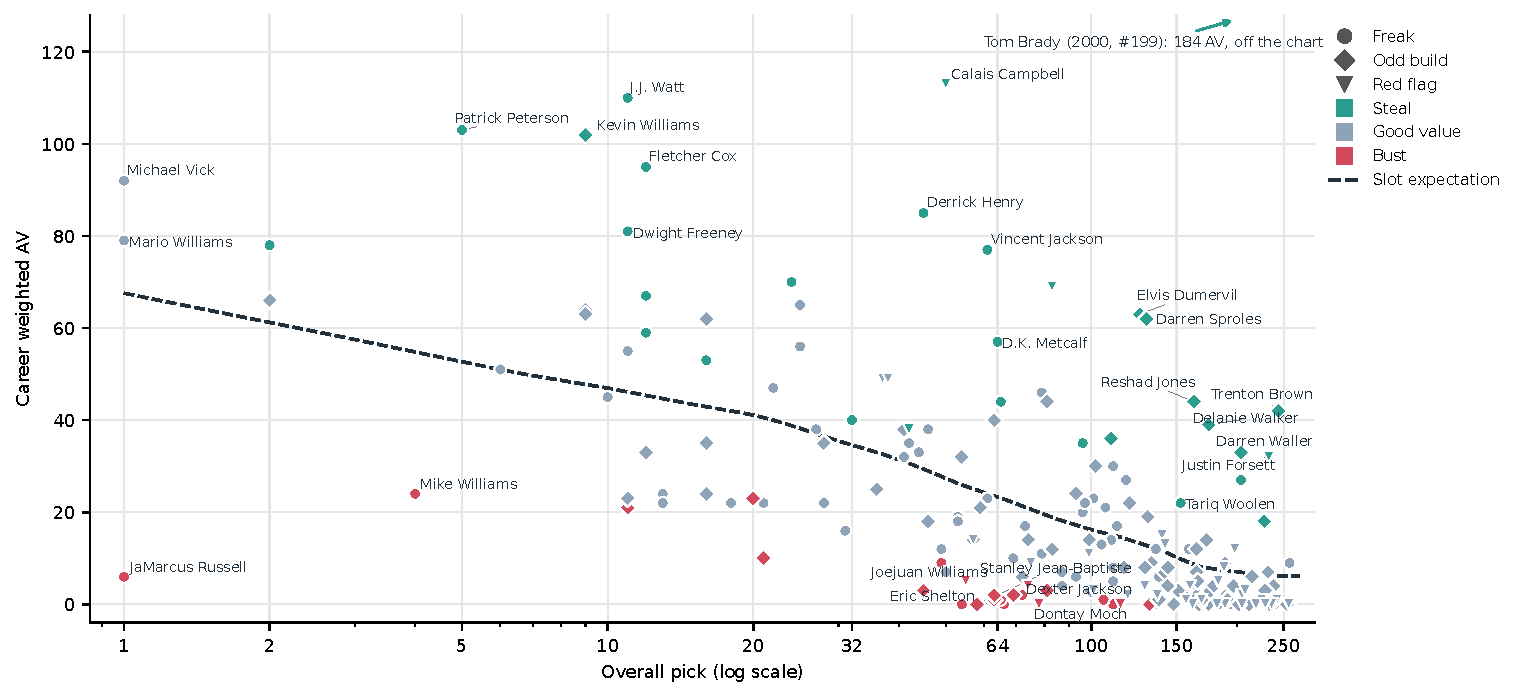
\includegraphics[width=0.92\linewidth]{figures/fig_unicorn_map.pdf}
\caption{Every drafted unicorn from the 2000--2022 classes. Marker shape gives the type, colour the grade. The dashed line is the position-neutral slot expectation; individual grades also use class and position adjustments, so a few points near the line are graded differently from their neighbours.}
\label{fig:map}
\end{figure}

\begin{table}[!htb]
\centering\footnotesize\sffamily
\begin{minipage}[t]{0.495\linewidth}
\centering
\caption{The 15 biggest unicorn steals by $z$.}
\label{tab:steals}
\setlength{\tabcolsep}{2.6pt}
\begin{tabular}{lll rr l rr r}
\toprule
Player & Pos & Type & Yr & Pk & Tm & AV & E & $z$\\
\midrule
\tabinput{tables/unicorn_steals_short.tex}
\bottomrule
\end{tabular}
\end{minipage}\hfill
\begin{minipage}[t]{0.495\linewidth}
\centering
\caption{The 15 biggest unicorn busts by $z$.}
\label{tab:busts}
\setlength{\tabcolsep}{2.6pt}
\begin{tabular}{lll rr l rr r}
\toprule
Player & Pos & Type & Yr & Pk & Tm & AV & E & $z$\\
\midrule
\tabinput{tables/unicorn_busts_short.tex}
\bottomrule
\end{tabular}
\end{minipage}

\vspace{3pt}{\scriptsize Type: F = Freak, O = Odd build, R = Red flag. Yr = draft class, Pk = overall pick, E = expected AV for the slot.}
\end{table}

Two things are worth noticing. The steals list holds two kinds of player. One is the Odd build or Red flag taken on day two or three (Brady, Campbell, Sproles, Waller, Dumervil, Trenton Brown, Reshad Jones, Forsett), where a low expectation makes a large multiple possible. The other is the Freak, either a slider (Vincent Jackson, Woolen, Metcalf, Henry) or a top-eleven pick who became a perennial All-Pro (Peterson, Watt). And the bust list cannot contain late picks by construction, so it is a list of first- and second-day disappointments, led by the most famous one in the sample.

\section{The team view}\label{sec:teams}

Table~\ref{tab:teams} and Figure~\ref{fig:teams} summarise each franchise's unicorn picks from 2000 to 2022.

\begin{figure}[!htb]
\centering
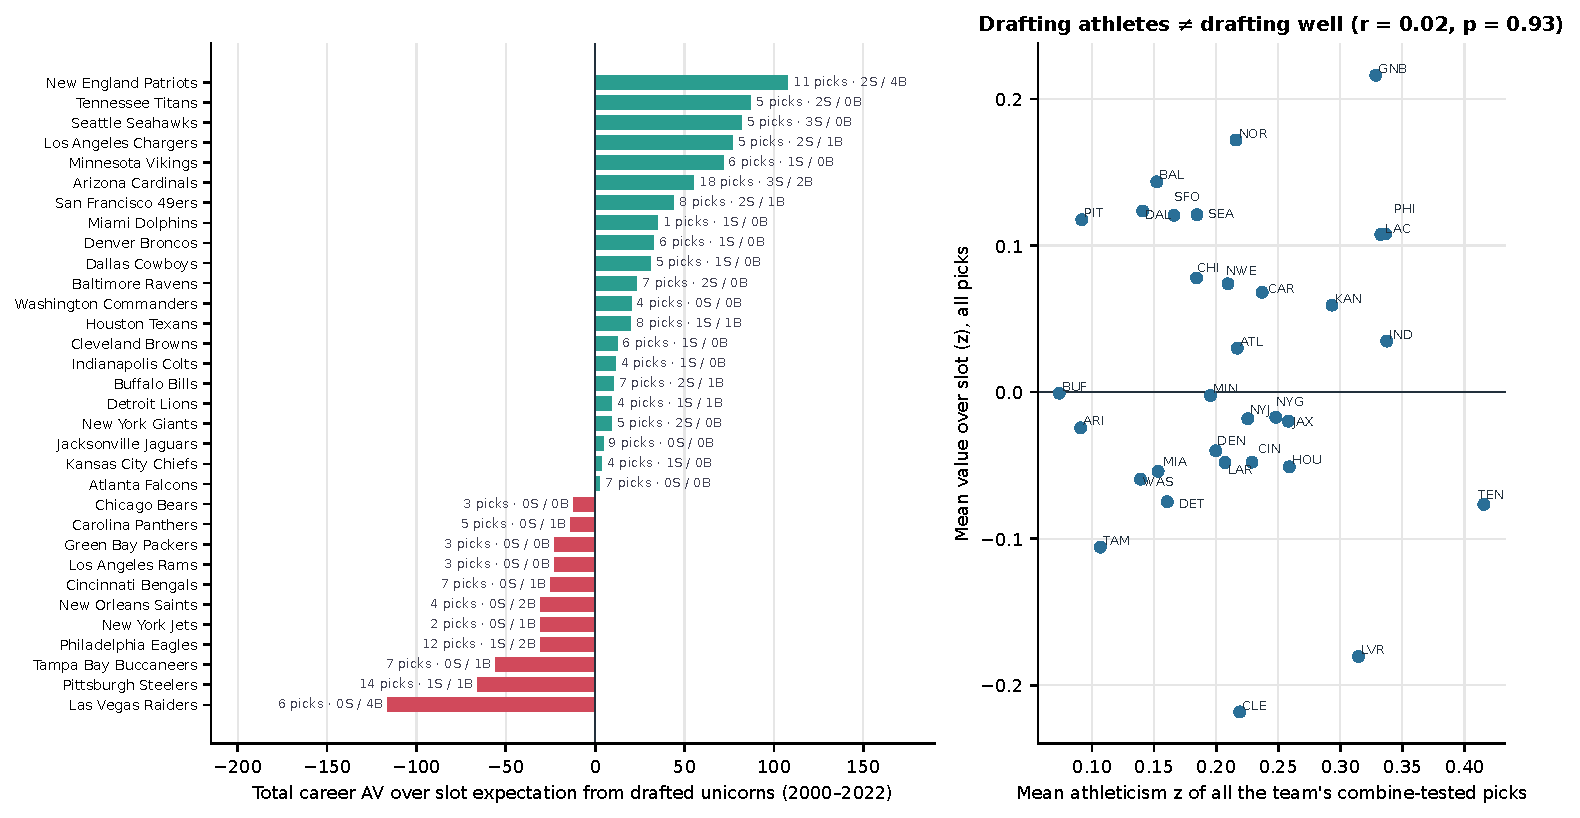
\includegraphics[width=0.94\linewidth]{figures/fig_teams.pdf}
\caption{Left: total career AV over slot expectation from each franchise's drafted unicorns, with pick, steal (S) and bust (B) counts. Right: for all of a team's combine-tested picks, average athleticism against average value over slot.}
\label{fig:teams}
\end{figure}

\begin{table}[!htb]
\centering\scriptsize\sffamily
\setlength{\tabcolsep}{3pt}
\caption{Unicorn picks by franchise, 2000--2022 classes. VOE = summed AV over slot. Best and worst are by $z$.}
\label{tab:teams}
\begin{tabular}{l rrrr rr ll}
\toprule
Franchise & Picks & Freaks & Steals & Busts & VOE & Mean $z$ & Best unicorn pick & Worst unicorn pick\\
\midrule
\tabinput{tables/teams.tex}
\bottomrule
\end{tabular}
\end{table}

Some observations a front office might draw from this, each with its caveat:

\begin{itemize}[leftmargin=1.4em]
\item \textbf{Appetite varies a great deal.} Arizona has drafted 18 unicorns, Pittsburgh 14, Philadelphia 12 and New England 11; Miami has drafted one and the Jets two. Arizona's haul includes Peterson, Campbell and Rodgers-Cromartie.
\item \textbf{New England's lead is one pick.} The Patriots top the table at $+108$ AV, but Brady alone is worth $+177$; their other ten unicorn picks sum to $-69$ and include four busts.
\item \textbf{Seattle has the best hit rate.} Three steals in five picks (Metcalf, Woolen, Forsett), all taken at pick 64 or later.
\item \textbf{The Raiders have the worst record.} Six unicorn picks, four busts (Russell, Bruce Campbell, Teyo Johnson, Demarcus Van Dyke) and $-116$ AV. The franchise's reputation for drafting stopwatch times over football players is visible in the data.
\end{itemize}

\textbf{Is any of this skill?} With between one and eighteen picks per team, mostly not demonstrably. If franchise labels are shuffled at random among the 201 unicorn picks, the spread of team mean $z$ is 0.58 on average; the observed spread is 0.62, a value exceeded in 30\% of shuffles. The team table is therefore best read as history, not as a ranking of unicorn-evaluation ability.

Nor does a general taste for athletes predict drafting success. Across the 32 franchises, the average athleticism of a team's draft picks is uncorrelated with the average value those picks returned over slot ($r=0.02$, $p=0.93$; right panel of Figure~\ref{fig:teams}). Green Bay and Tennessee both draft unusually athletic classes; one sits at the top of the value axis and the other below average.

\section{Robustness}\label{sec:robust}

\begin{table}[!htb]
\centering\footnotesize\sffamily
\setlength{\tabcolsep}{3.4pt}
\caption{Sensitivity of the main result to the unicorn definition. Each row re-flags the sample; outcome columns are for drafted, graded players of each type.}
\label{tab:sens}
\begin{tabular}{l rrrr rrrr rrrr}
\toprule
 & \multicolumn{4}{c}{Freak} & \multicolumn{4}{c}{Odd build} & \multicolumn{4}{c}{Red flag}\\
\cmidrule(lr){2-5}\cmidrule(lr){6-9}\cmidrule(lr){10-13}
Definition & $n$ & $z$ & Steal & Bust & $n$ & $z$ & Steal & Bust & $n$ & $z$ & Steal & Bust\\
\midrule
\tabinput{tables/sensitivity.tex}
\bottomrule
\end{tabular}
\end{table}


\textbf{Threshold and detector.} Whether the cut is 2\%, 5\% or 10\%, and whether we use the consensus or any single detector or view, Freaks land between $+0.05$ and $+0.19$ SD above slot with a bootstrap interval that includes zero every time (Table~\ref{tab:sens}). Their steal rate is 16--21\% and their bust rate 9--17\% across all eight definitions. The conclusion does not depend on the modelling choices.

\textbf{Red flags are fragile.} Their mean flips sign across definitions, depending on whether Brady is in the flagged set. No conclusion should be drawn about them beyond ``rarely drafted''.

\textbf{Imputation.} Restricting to players who completed at least five of six drills gives a Freak mean of $+0.21$ ($n=57$) against $+0.04$ for typical players: slightly larger, same sign, same overlap with zero.

\textbf{Unfinished careers.} Restricting to the 2000--2018 classes, whose careers are largely complete, gives $+0.10$ for Freaks ($n=69$; 20\% steals, 13\% busts) against $+0.01$ for typical players (18\% and 15\%).

\section{Discussion}\label{sec:discuss}

\subsection{What a front office should take from this}

\begin{enumerate}[leftmargin=1.4em]
\item \textbf{Do not expect a discount, or fear a trap.} On average the market for freak athletes clears at about the right price. A team that drafts one at the slot the league assigns is making a fair bet.
\item \textbf{Athleticism is slightly under-priced; rarity is not priced at all.} The one continuous signal that survives controls is the athleticism composite. Being \emph{different} adds nothing once \emph{better} is accounted for. A draft model should carry a size-adjusted athletic score, not an anomaly score.
\item \textbf{When the consensus puts a Freak in round one, the floor is high.} A 7\% bust rate over 27 picks, against 23\% for other first-rounders, is the largest practical difference in the study. It is a subgroup result and needs out-of-sample confirmation, but it argues against the instinct to fade the ``workout warrior'' at the top of the board.
\item \textbf{Be sceptical of rare size without rare movement.} Odd builds on day two and outsized tackles have the worst records. Mass is the easiest kind of rarity to see and the least reliable.
\item \textbf{A Freak who is still available on day three is usually available for a reason.} Late-round Freaks have under-performed ordinary late-round picks on steal rate.
\item \textbf{Use the detector for triage and for data hygiene.} The same pipeline that flags unicorns flagged every mislabelled row in the source data. Run on a scouting database, it is a cheap way to find both the prospects who deserve a second look and the records that need correcting.
\end{enumerate}

\subsection{Limitations}\label{sec:limits}

\textbf{Athletic testing only.} There is no college production, usage, age, medical or character information here. A prospect whose rarity is in how he was used is invisible to this model. The pipeline accepts additional columns without modification: adding dominator rating, target share or depth of target to the feature vector for skill positions, from a source such as the CollegeFootballData API, would extend it to production unicorns.

\textbf{Approximate Value is blunt.} It under-rates positions with few counting statistics and rewards longevity. The position multiplier absorbs average differences but not everything; a tight end's 40 AV and a guard's are not the same achievement.

\textbf{Value is not surplus value.} We compare production with slot expectation, not with salary. Under the rookie wage scale a first-round hit carries more surplus than this analysis credits, and Massey and Thaler's \cite{massey} finding that top picks are over-valued relative to their cost is not tested here.

\textbf{Selection.} Only players who attended the combine (or a 2021 pro day) and ran a 40 are in the sample. Prospects who skipped the 40 entirely are excluded, and they are disproportionately elite. Drafted Red flags are a heavily selected sub-sample.

\textbf{Recent classes.} The class factor rescales unfinished careers but cannot know their shape: early AV favours high picks, who play immediately. The 2019--2022 grades are provisional.

\textbf{Position labels} are those listed at the combine. A handful of players are graded at a position they did not play (Darren Waller and Delanie Walker appear as receivers; Kevin Williams as an edge defender).

\textbf{Equal drill weights.} The athleticism composite weights the six drills equally, which occasionally types a player on the strength of jumps despite a poor 40. Position-specific weights are a natural refinement.

\textbf{Multiple comparisons.} The round, position and archetype breakdowns involve dozens of cells. A few will look striking by chance. Prior work also finds that combine results explain little NFL performance once draft position is known \cite{kuzmits,robbins,berri}, which is consistent with our small overall effects.

\section{Conclusion and a watch list}

Unsupervised learning is well suited to the first half of the unicorn question. Three detectors, two views and a few lines of robust statistics recover the players scouts would name from memory and a good many they would not, without ever being told who succeeded. The second half, whether rarity is worth paying for, turns out to have an unglamorous answer: across 23 gradeable draft classes, teams that drafted freak athletes got, on average, what they paid for. The edges are at the margins: trust the confirmed first-round Freak a little more than the league does, and the oversized or oddly built day-two pick a little less.

The model also flags players from classes too young to grade. Table~\ref{tab:recent} lists the Freaks from 2023 onward as an out-of-sample test: if the pattern above holds, the first-rounders among them should bust less often than their draft-day peers.

\begin{table}[!htb]
\centering\small\sffamily
\caption{Freak unicorns from the 2023--2026 classes (not yet gradeable). Draft slots for 2026 are matched by name from the draft file.}
\label{tab:recent}
\begin{tabular}{ll r rrr r rl}
\toprule
Player & Pos & Class & Ht & Wt & 40 & Ath & Pick & Team\\
\midrule
\tabinput{tables/recent.tex}
\bottomrule
\end{tabular}
\end{table}

\appendix
\section{Reproducibility}

The replication package contains six scripts, run in order by \texttt{run\_all.sh}:

\begin{center}\small\sffamily
\begin{tabular}{ll}
\toprule
\texttt{01\_prepare.py} & Load \texttt{nflverse} files, parse heights, resolve positions, remove namesakes\\
\texttt{02\_detect.py} & Imputation, size/era adjustment, three detectors, two views, consensus, typing\\
\texttt{03\_value.py} & Slot curve, class and position factors, VOE, $z$, grades\\
\texttt{04\_analysis.py} & All statistics, tests, regressions, clustering, team tables\\
\texttt{05\_figures.py} & All figures\\
\texttt{06\_tables.py} & Remaining \LaTeX\ tables\\
\bottomrule
\end{tabular}
\end{center}

Random seeds are fixed, so the pipeline reproduces every number in this paper from the three downloaded CSV files. The file \texttt{all\_unicorns.csv} lists all 390 flagged players with their measurements, scores, type, draft slot, value and grade. The core of the detection step, for one position group, is:

\begin{lstlisting}
# X: imputed [ht, wt, forty, bench, vertical, broad_jump, cone, shuttle] for one position
A = np.column_stack([np.ones(n), X.ht, X.wt, X.wt**2, year - 2013, year == 2021])
for d in drills:                                   # size- and era-adjust each drill
    obs  = raw[d].notna().values                   # fit only on players who ran it
    beta = np.linalg.lstsq(A[obs], X[d][obs], rcond=None)[0]
    res  = X[d] - A @ beta
    med  = np.median(res[obs]); mad = 1.4826 * np.median(np.abs(res[obs] - med))
    sub["adj_" + d] = sign[d] * (res - med) / mad  # positive = better than size predicts

views = {"full": ["z_ht", "z_wt"] + ["adj_" + d for d in drills],
         "core": ["z_ht", "z_wt", "adj_forty"]}
for v, cols in views.items():
    F = sub[cols].values
    s_if  = -IsolationForest(n_estimators=500, random_state=42).fit(F).score_samples(F)
    s_lof = -LocalOutlierFactor(n_neighbors=35).fit(F).negative_outlier_factor_
    s_md  = np.sqrt(MinCovDet(support_fraction=0.85, random_state=42).fit(F).mahalanobis(F))
    pct   = [rankdata(s) / n for s in (s_if, s_lof, s_md)]
    sub["cons_" + v] = rankdata(np.mean(pct, axis=0)) / n

sub["consensus"] = rankdata(sub[["cons_full", "cons_core"]].max(axis=1)) / n
sub["unicorn"]   = sub.consensus > 0.95
\end{lstlisting}

\begin{thebibliography}{99}\footnotesize\setlength{\itemsep}{1pt}
\bibitem{nflverse} Carl, S., Baldwin, B., Sharpe, L., Ho, T., and Edwards, J. \emph{nflverse: open-source NFL data} (combine, draft\_picks and players releases). \url{https://github.com/nflverse/nflverse-data}.
\bibitem{drinen} Drinen, D. Approximate Value. \emph{Pro-Football-Reference.com}. \url{https://www.pro-football-reference.com/about/approximate_value.htm}.
\bibitem{iforest} Liu, F.~T., Ting, K.~M., and Zhou, Z.-H. (2008). Isolation Forest. \emph{Proceedings of the Eighth IEEE International Conference on Data Mining}, 413--422.
\bibitem{lof} Breunig, M.~M., Kriegel, H.-P., Ng, R.~T., and Sander, J. (2000). LOF: Identifying density-based local outliers. \emph{Proceedings of the ACM SIGMOD International Conference on Management of Data}, 93--104.
\bibitem{mcd} Rousseeuw, P.~J., and Van Driessen, K. (1999). A fast algorithm for the minimum covariance determinant estimator. \emph{Technometrics}, 41(3), 212--223.
\bibitem{mice} van Buuren, S., and Groothuis-Oudshoorn, K. (2011). mice: Multivariate imputation by chained equations in R. \emph{Journal of Statistical Software}, 45(3), 1--67.
\bibitem{lowess} Cleveland, W.~S. (1979). Robust locally weighted regression and smoothing scatterplots. \emph{Journal of the American Statistical Association}, 74(368), 829--836.
\bibitem{sklearn} Pedregosa, F., et al. (2011). Scikit-learn: Machine learning in Python. \emph{Journal of Machine Learning Research}, 12, 2825--2830.
\bibitem{massey} Massey, C., and Thaler, R.~H. (2013). The loser's curse: Decision making and market efficiency in the National Football League draft. \emph{Management Science}, 59(7), 1479--1495.
\bibitem{kuzmits} Kuzmits, F.~E., and Adams, A.~J. (2008). The NFL Combine: Does it predict performance in the National Football League? \emph{Journal of Strength and Conditioning Research}, 22(6), 1721--1727.
\bibitem{robbins} Robbins, D.~W. (2010). The National Football League (NFL) Combine: Does normalized data better predict performance in the NFL draft? \emph{Journal of Strength and Conditioning Research}, 24(11), 2888--2899.
\bibitem{berri} Berri, D.~J., and Simmons, R. (2011). Catching a draft: On the process of selecting quarterbacks in the National Football League amateur draft. \emph{Journal of Productivity Analysis}, 35(1), 37--49.
\end{thebibliography}

\end{document}
